% %
% LAYOUT_E.TEX - Short description of REFMAN.CLS
%                                       99-03-20
%
%  Updated for REFMAN.CLS (LaTeX2e)
%
\documentclass[twoside,a4paper]{refart}
\usepackage{makeidx}
\usepackage{ifthen}
% ifthen wird vom Bild von N.Beebe gebraucht!

\usepackage[utf8]{inputenc}
\usepackage[spanish]{babel}

% sin este no se pueden incluir imagenes
\usepackage{graphicx}


% hipervinculos a internet
\usepackage{url}

\def\bs{\char'134 } % backslash in \tt font.
\newcommand{\ie}{i.\,e.,}
\newcommand{\eg}{e.\,g..}
\DeclareRobustCommand\cs[1]{\texttt{\char`\\#1}}

\title{Interfaz gráfica [nombre pendiente]}
\author{Patricia González Gaspar\\
Miguel Landa\\
Julio\\
H27.0 --- Version 1}

\date{}
\emergencystretch1em  %

\pagestyle{myfootings}
\markboth{Interfaz gráfica [nombre pendiente]}%
         {Interfaz gráfica [nombre pendiente]}

\makeindex 

\setcounter{tocdepth}{2}

%%%%%%%%%%%%%%%%%%%%%%%%%%%%%%%%%%%%%%%%%%%%%%%%%%%%%%%%%%%%%%%%%%%%%%
%%%%%%%%%%%%%%%%%%%%%%%%%%%%%%%%%%%%%%%%%%%%%%%%%%%%%%%%%%%%%%%%%%%%%%
%%%%%%%%%%%%%%%%%%%%%%%%%%%%%%%%%%%%%%%%%%%%%%%%%%%%%%%%%%%%%%%%%%%%%%
%%%%%%%%%%%%%%%%%%%%%%%%%%%%%%%%%%%%%%%%%%%%%%%%%%%%%%%%%%%%%%%%%%%%%%

\begin{document}

\maketitle

\begin{abstract}
    Este software realiza análisis de estacionariedad de escala amplia
    mediante una interfaz gráfica intuitiva, diseñada para su uso por
    personal sin una formación amplia en programación.
    Este software está escrito en \texttt{python 3} y algunas partes en \texttt{R}. 
\end{abstract}


Aquí va la introducción.

\tableofcontents

\newpage

%%%%%%%%%%%%%%%%%%%%%%%%%%%%%%%%%%%%%%%%%%%%%%%%%%%%%%%%%%%%%%%%%%%%%%

\section{Prerequisitos}
\index{Prerequisitos}

Para el correcto funcionamiento de este software, se requiere la instalación de algunas 
librerías correspondientes a dos lenguajes de programación (\texttt{python 3}, \texttt{R})
y a la su coordinación.
%
Se recomienda instalar los siguientes programas en el orden indicado:

\marginlabel{R:}
El software estadístico \texttt{R} puede descargarse desde su página oficial \url{https://www.r-project.org/}. 
%
A menos que se use un equipo de cómputo muy viejo, es recomendable usar la versión 
\texttt{x64}.

\marginlabel{Anaconda:} 
Contiene una dsitribución del lenguaje \texttt{python} junto a una gran variedad de
librerías para cómputo científico.
%
Su instalación es sencilla, si bien un poco tardada.
%
Puede descargarse desde su página oficial \url{https://www.anaconda.com/download/}

\attention
Debido a motivos históricos, el lenguaje de programación \texttt{python} mantiene activas
las versiones 2 y 3; para el correcto funcionamiento de este software es necesario usar
la versión \textbf{3}.
\nopagebreak
\begin{maxipage}
Es muy importante que registre o recuerde la carpeta donde se ha instalado Anaconda y R, ya
que esta información será usada durante la instalación.
\end{maxipage}\nopagebreak


%%%%%%%%%%%%%%%%%%%%%%%%%%%%%%%%%%%%%%%%%%%%%%%%%%%%%%%%%%%%%%%%%%%%%%

\section{Instalación}

%\subsection{General}

\marginlabel{Instalación de paquetes:}
Lance el programa \texttt{Anaconda Navigator} como `Administrador'. 
%
Una vez abierto el programa, siga las instrucciones para instalar paquetes:
\begin{enumerate}
\item Abrir la pestaña `Enviroments' en la parte izquierda de la pantalla.
\item Ubicar el menú desplegable de la parte superior con la opción `Installed' y 
cambiarlo a la opción `All'.
\item En la barra de búsqueda, ingresar el nombre del paquete a instalar.
\item Marcar el recuadro a la izquierda del paquete a instalar.
\item Para efectuar la instalación, seleccionar el botón `Apply' en la esquina 
inferior derecha.
\end{enumerate}
A continuación se listan los paquetes a instalarse:
\begin{itemize}
\item \texttt{pyqtgraph}
\item \texttt{rpy2}
\end{itemize}

\attention
De no usarse Anaconda como `Administrador' es posible que algunas librerías se instalen
sólo de forma temporal.

\marginlabel{Código de la interfaz:}
La carpeta `Interfaz' puede ser \textit{colocada} en cualquier otra carpeta del disco duro.
%
Es recomendable recordar tal ubicación o crear un acceso directo desde `Escritorio'.

\begin{fullpage}
\begin{figure}
\centering
\caption{Instalación de paquetes usando Anaconda.}
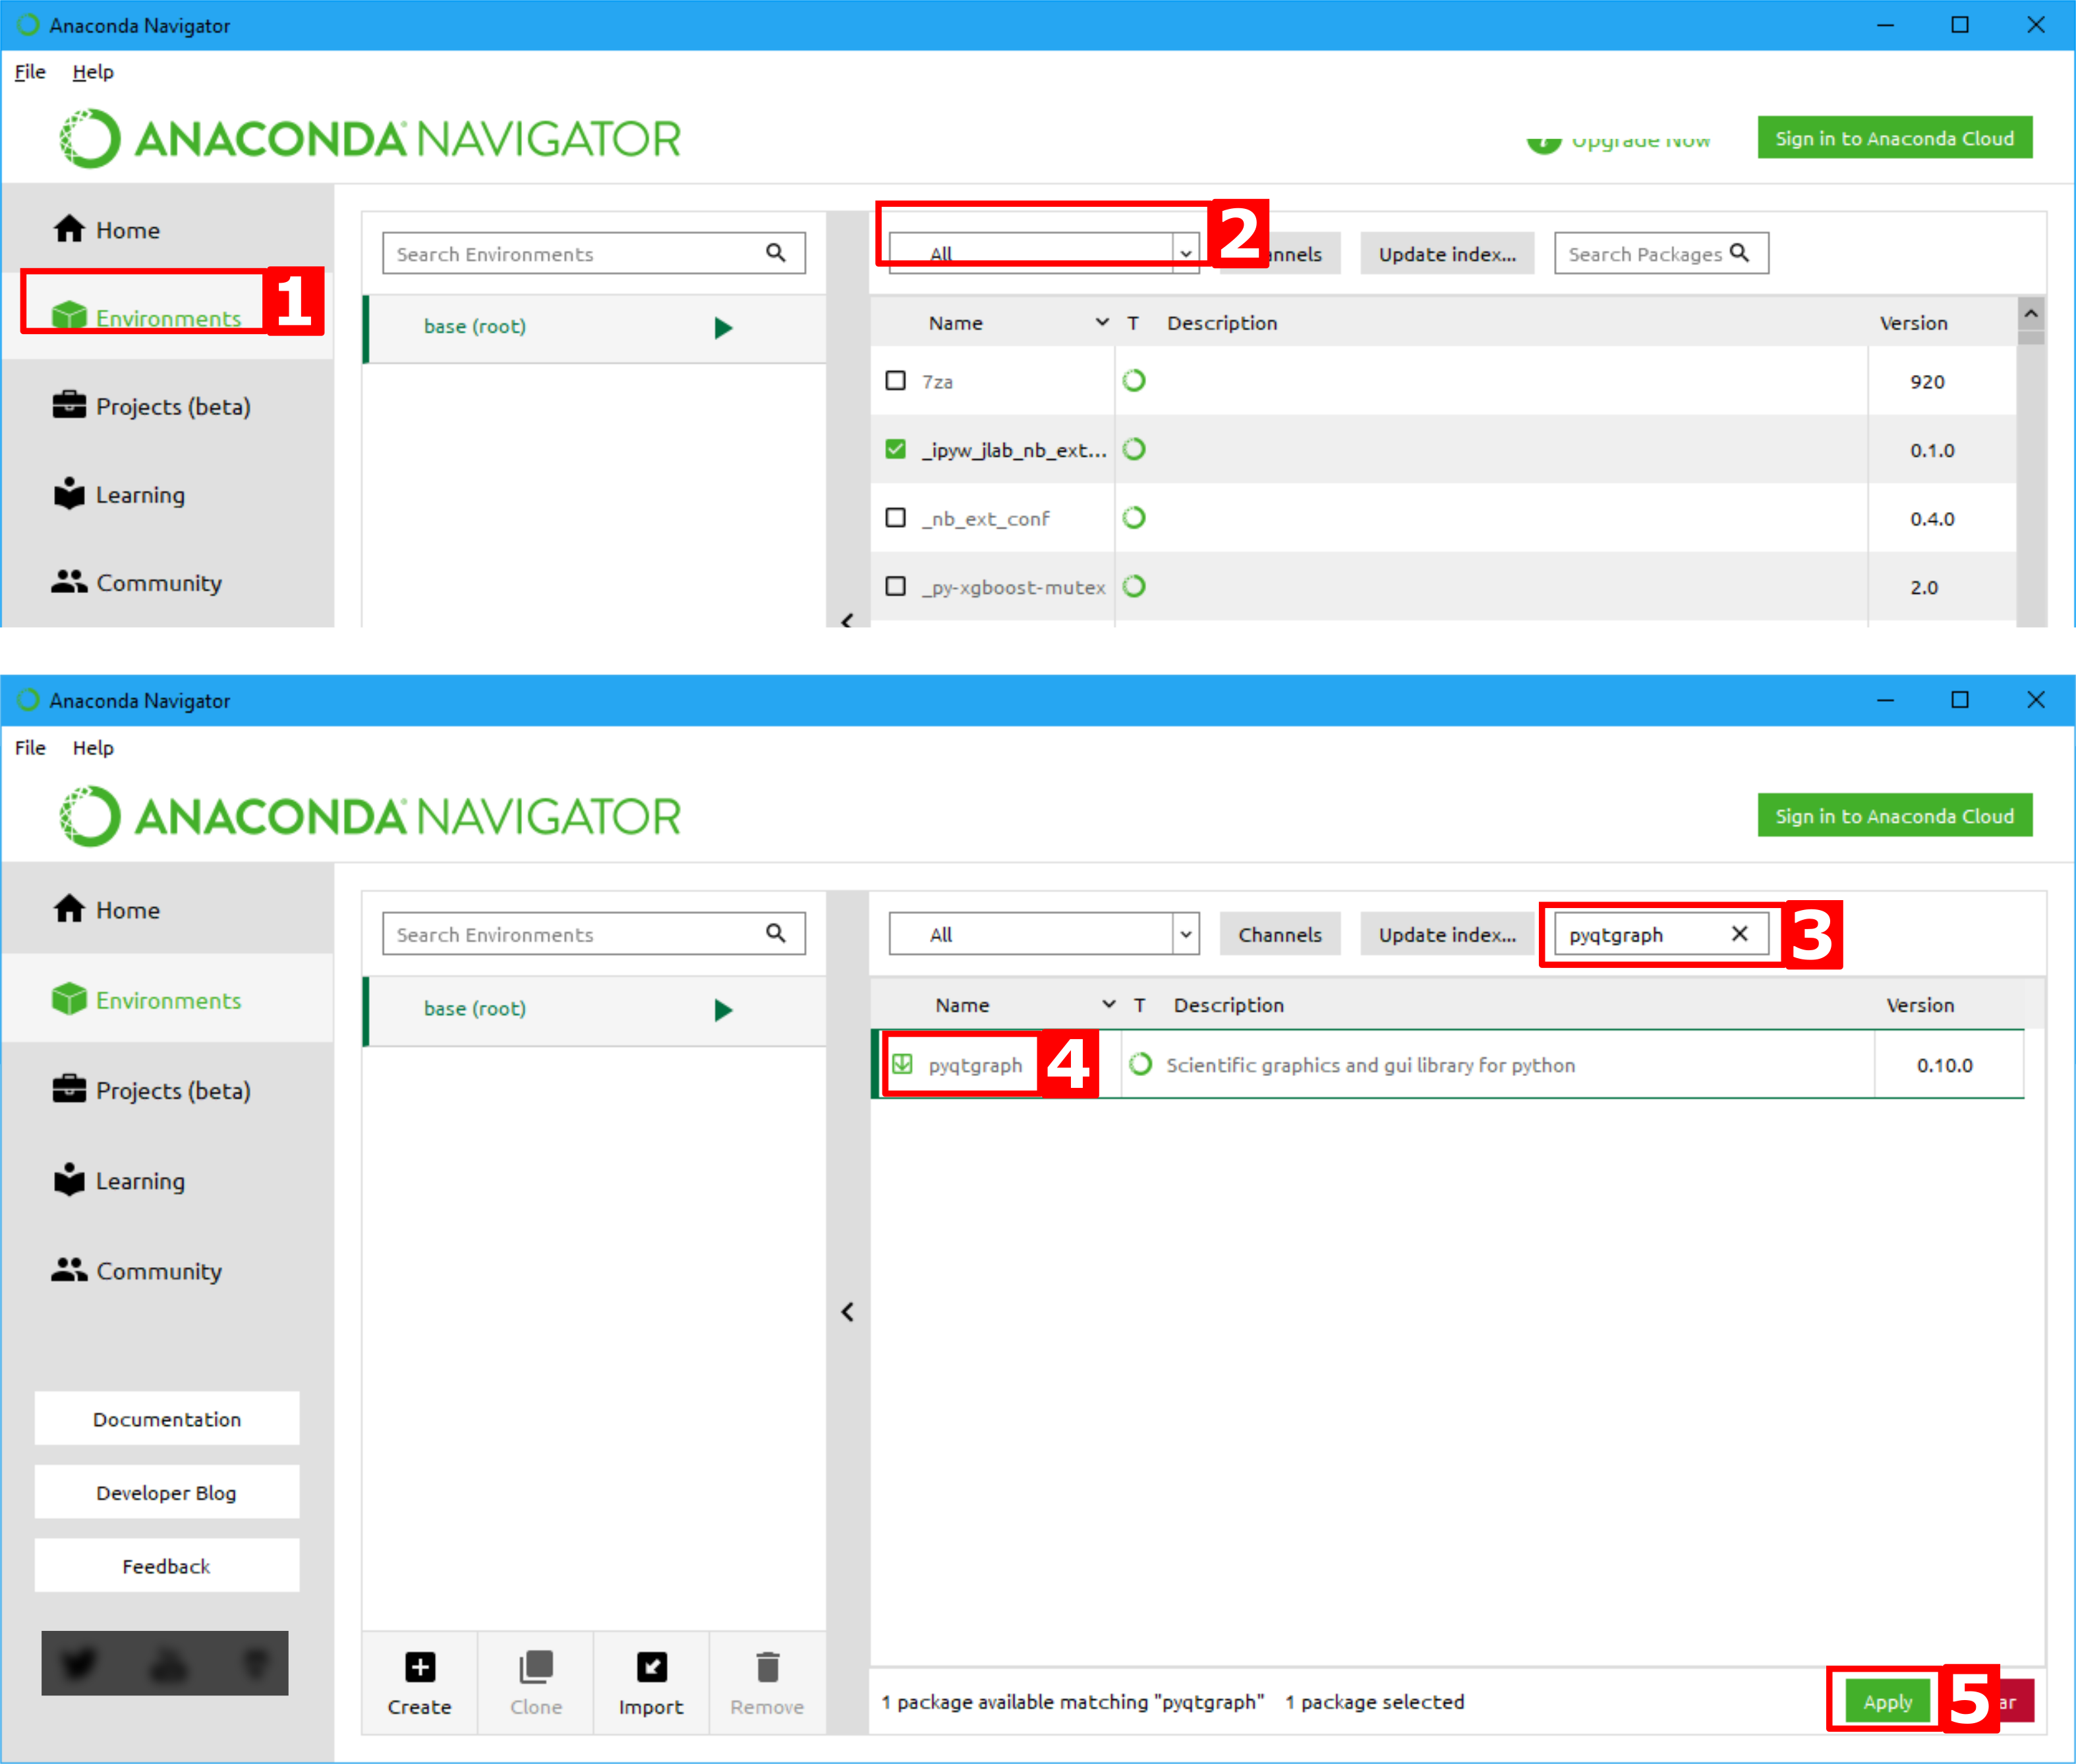
\includegraphics[width=0.8\linewidth]{./imagenes/anaconda_paquetes.png}
\end{figure}
\end{fullpage}

%\subsection*{Windows 10}

\marginlabel{Creación de variables \texttt{path}:}
sadasd

%%%%%%%%%%%%%%%%%%%%%%%%%%%%%%%%%%%%%%%%%%%%%%%%%%%%%%%%%%%%%%%%%%%%%%

\section{Log de cambios}

%%%%%%%%%%%%%%%%%%%%%%%%%%%%%%%%%%%%%%%%%%%%%%%%%%%%%%%%%%%%%%%%%%%%%%

\printindex

\end{document}
